
% This LaTeX was auto-generated from MATLAB code.
% To make changes, update the MATLAB code and republish this document.

\documentclass{article}
\usepackage{graphicx}
\usepackage{color}

\sloppy
\definecolor{lightgray}{gray}{0.5}
\setlength{\parindent}{0pt}

\begin{document}

    
    
\subsection*{Contents}

\begin{itemize}
\setlength{\itemsep}{-1ex}
   \item DSP Homework 5 Problem 3 6.3-8
   \item DSP Hoework 5 Problem 5 6.5-2
   \item DSP Homework 5 PRoblem 9 7.7-2
\end{itemize}


\subsection*{DSP Homework 5 Problem 3 6.3-8}

\begin{verbatim}
T3 = 1/10;

omega3 = -pi:.01:pi;

Hz3 = @(z) T3/2.*(1+z.^-1)./(1-z.^-1);

plot(omega3, abs(Hz3(exp(j.*omega3))));
xlabel('Frequency (Omega)');
title('Magnitude of H(jw) from H(Z)');
axis([-pi pi 0 20]);
figure;
plot(omega3, angle(Hz3(exp(j.*omega3))));
xlabel('Frequency (Omega)');
title('Angle of H(jw) from H(Z)');
axis([-pi pi -pi pi]);

% Part A
Xz3a = @(z) z.*(z-.995)./(z.^2 - 1.99*z + 1)

figure;
plot(omega3, abs(Hz3(exp(j.*omega3)).*Xz3a(exp(j.*omega3))));
xlabel('Frequency (Omega)');
title('Magnitude of H(w)*Xa(w) from H(Z)');
axis([-pi pi 0 20]);
figure;
plot(omega3, angle(Hz3(exp(j.*omega3)).*Xz3a(exp(j.*omega3))));
xlabel('Frequency (Omega)');
title('Angle of H(w)*Xa(w) from H(Z)');
axis([-pi pi -pi pi]);

% Part B
Xz3b = @(z) .5*z./(z.^2 - 1.732*z + 1)

figure;
plot(omega3, abs(Hz3(exp(j.*omega3)).*Xz3b(exp(j.*omega3))));
xlabel('Frequency (Omega)');
title('Magnitude of H(w)*Xb(w) from H(Z)');
axis([-pi pi 0 50]);
figure;
plot(omega3, angle(Hz3(exp(j.*omega3)).*Xz3b(exp(j.*omega3))));
xlabel('Frequency (Omega)');
title('Angle of H(w)*Xb(w) from H(Z)');
axis([-pi pi -pi pi]);

% Part C
Xz3c = @(z) z.^2./(z.^2 + 1)

figure;
plot(omega3, abs(Hz3(exp(j.*omega3)).*Xz3c(exp(j.*omega3))));
xlabel('Frequency (Omega)');
title('Magnitude of H(w)*Xc(w) from H(Z)');
axis([-pi pi 0 50]);
figure;
plot(omega3, angle(Hz3(exp(j.*omega3)).*Xz3c(exp(j.*omega3))));
xlabel('Frequency (Omega)');
title('Angle of H(w)*Xc(w) from H(Z)');
axis([-pi pi -pi pi]);
\end{verbatim}

        \color{lightgray} \begin{verbatim}
Xz3a =

  function_handle with value:

    @(z)z.*(z-.995)./(z.^2-1.99*z+1)


Xz3b =

  function_handle with value:

    @(z).5*z./(z.^2-1.732*z+1)


Xz3c =

  function_handle with value:

    @(z)z.^2./(z.^2+1)

\end{verbatim} \color{black}
    
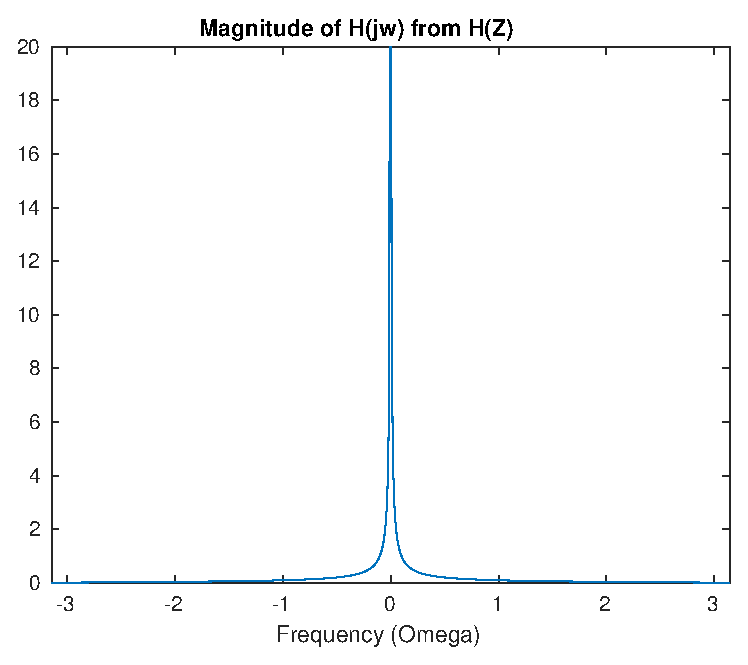
\includegraphics [width=4in]{hw5_01.eps}

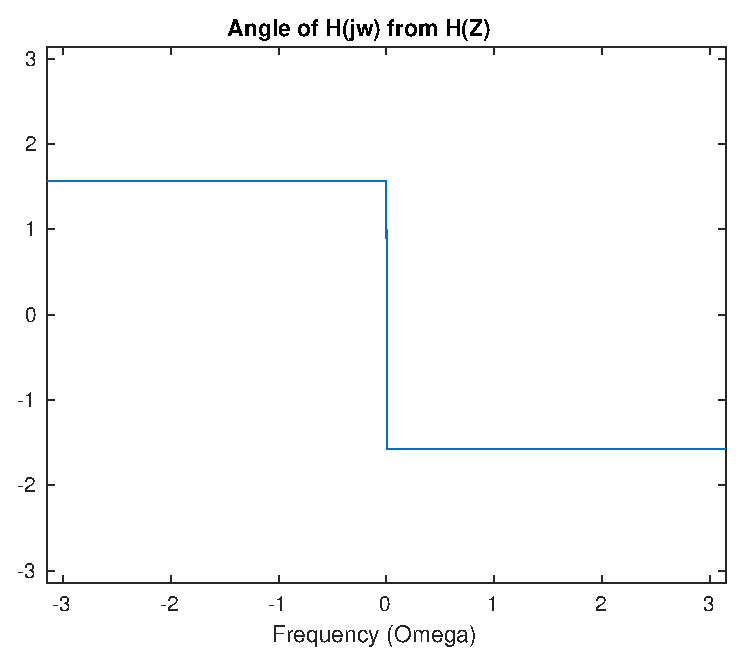
\includegraphics [width=4in]{hw5_02.eps}

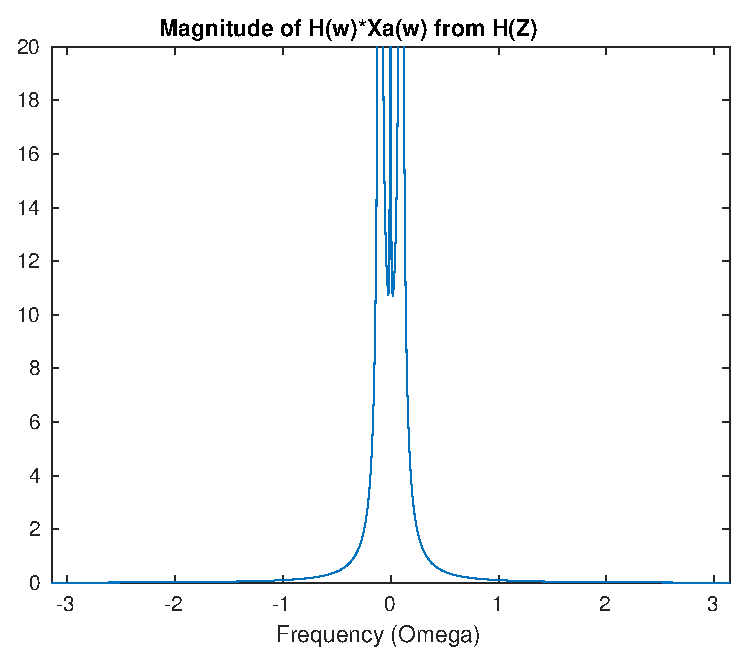
\includegraphics [width=4in]{hw5_03.eps}

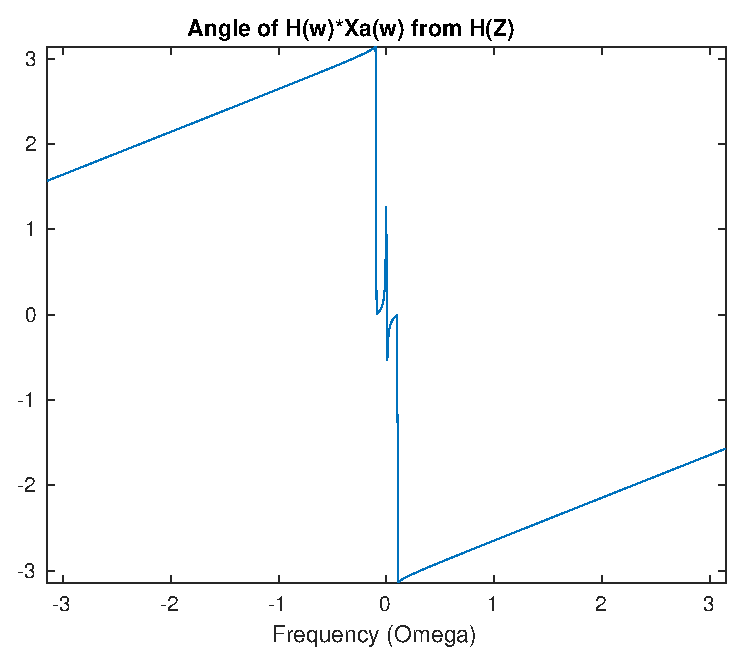
\includegraphics [width=4in]{hw5_04.eps}

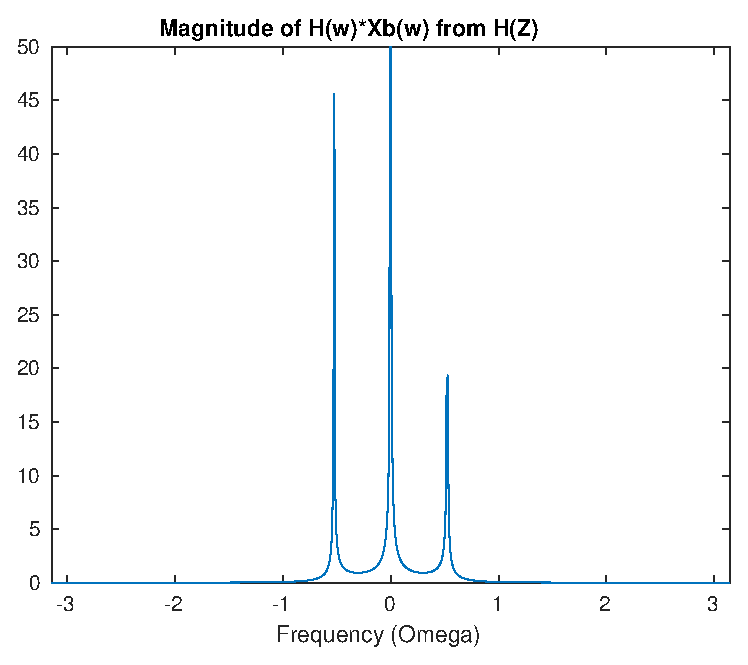
\includegraphics [width=4in]{hw5_05.eps}

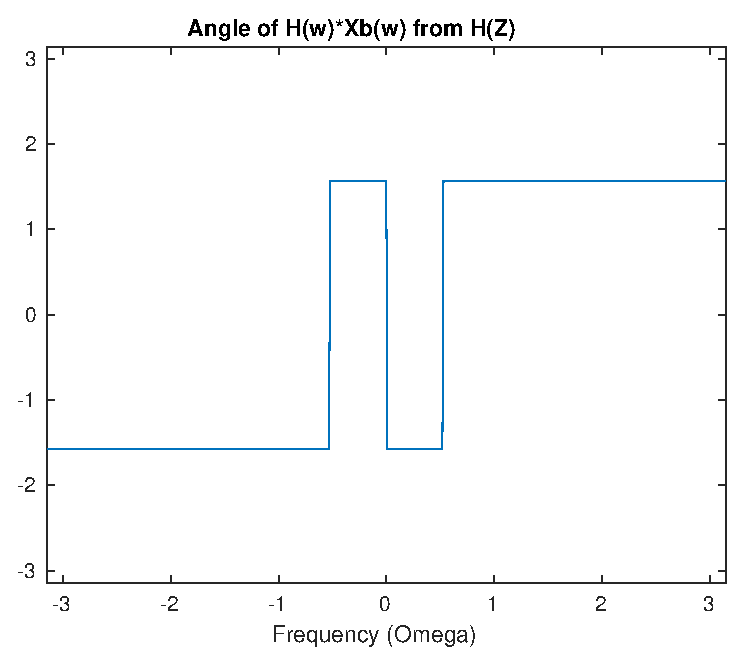
\includegraphics [width=4in]{hw5_06.eps}

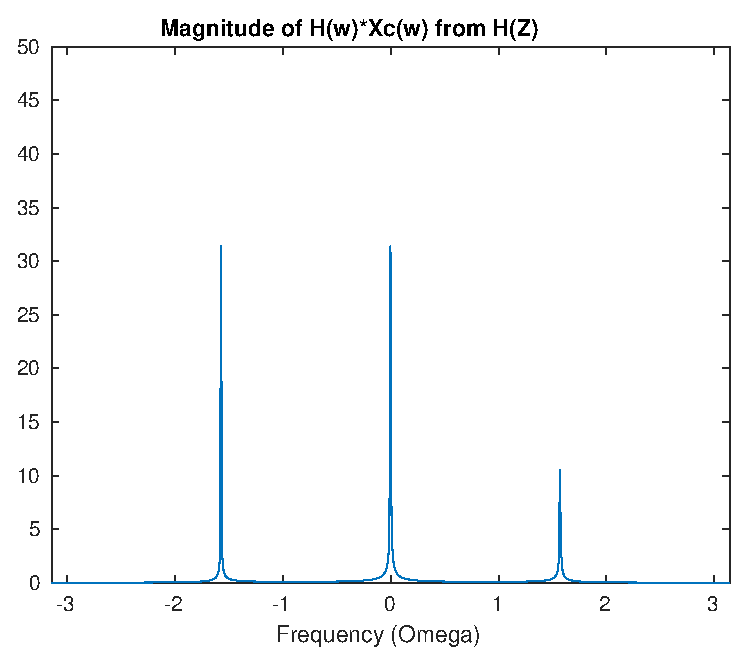
\includegraphics [width=4in]{hw5_07.eps}

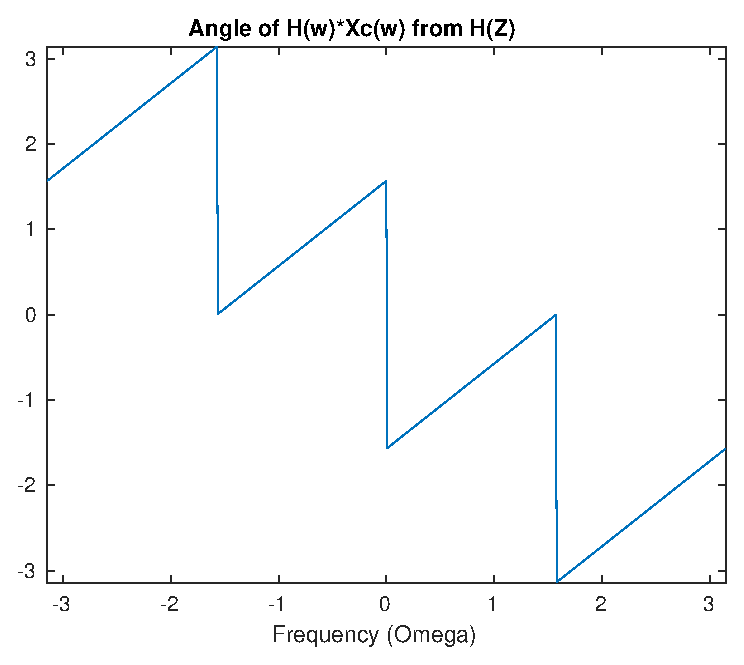
\includegraphics [width=4in]{hw5_08.eps}


\subsection*{DSP Hoework 5 Problem 5 6.5-2}

\begin{verbatim}
t5 = 0:.00001:.001;
B5 = 10000*pi;
T5 = 10^-4;
omega5 = 1:1:1/(T5);

% Part A

xc5 = @(t) sinc(B5*t/pi);
Xc5 = @(omega) T5*(heaviside(omega)-heaviside(omega-1/(T5*2)));

figure;
plot(t5, xc5(t5));
xlabel('Time (s)');
title('Input Signal to C/D');
figure;
plot(omega5, abs(Xc5(omega5)));
xlabel('Frequency (omega)');
title('Input Spectra to C/D');
% figure;
% plot(omega5, angle(Xc5(omega5)));
% xlabel('Frequency (omega)');
% ylabel('Angle (rads)');
% title('Input Spectra to C/D');

% Part B
n5 = 0:1:10;
xd5 = @(n5) sinc(B5*n5*T5/pi);

figure;
stem(n5, xd5(n5));
xlabel('Samples');
title('Input signal for H(Omega)');

Omega5 = -pi:.01:pi;
X5 = @(Omega5) pi* (heaviside(Omega5 + pi/2) - heaviside(Omega5 - pi/2));

figure;
plot(Omega5, abs(X5(Omega5)));
xlabel('Frequency (Omega))');
title('Input Spectra for H(Omega)');
% figure;
% plot(Omega5, angle(Xd5(Omega5)));
% xlabel('Frequency (Omega))');
% title('Input Spectra for H(Omega)');

% Part C
H5 = @(Omega5) j*Omega5/T5;
Y5 = @(Omega5) X5(Omega5).*H5(Omega5);

figure;
plot(Omega5, abs(Y5(Omega5)));
xlabel('Frequency (Omega)');
title('Output Spectra for H(Omega)');
figure;
plot(Omega5, angle(Y5(Omega5)));
xlabel('Frequency (Omega)');
ylabel('Angle (rads)');
title('Output Spectra angle for H(Omega)');

yd5 = @(n5) 1/(2*pi*T5).*(pi.*n5.*cos(pi*n5/2) - 2*sin(pi*n5/2))./n5.^2;

figure;
stem(n5, yd5(n5));
xlabel('Samples');
ylabel('Amplitude');
title('Output signal for H(Omega)');

% Part D

yc5 = @(t) yd5(t/T5);

figure;
plot(t5, yc5(t5));
xlabel('Time (s)');
ylabel('Amplitude');
title('Output signal');
\end{verbatim}

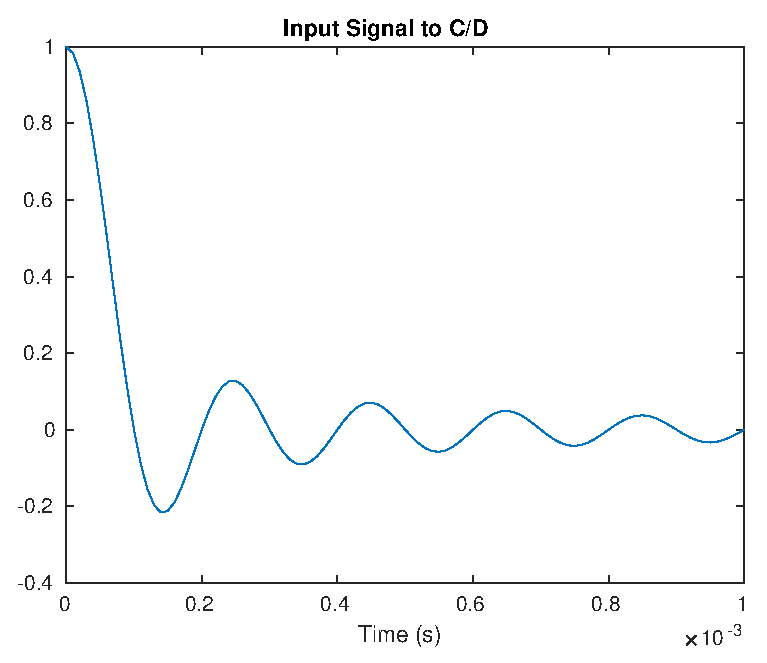
\includegraphics [width=4in]{hw5_09.eps}

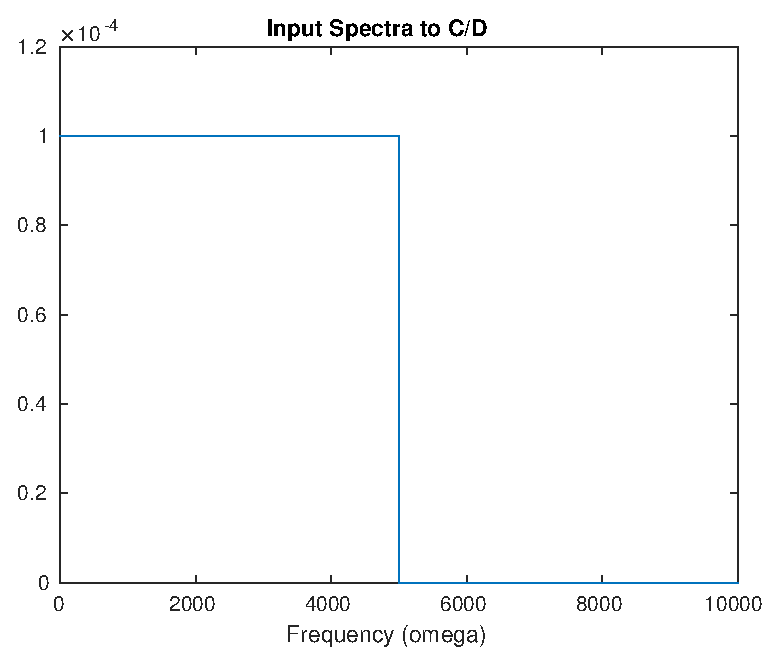
\includegraphics [width=4in]{hw5_10.eps}

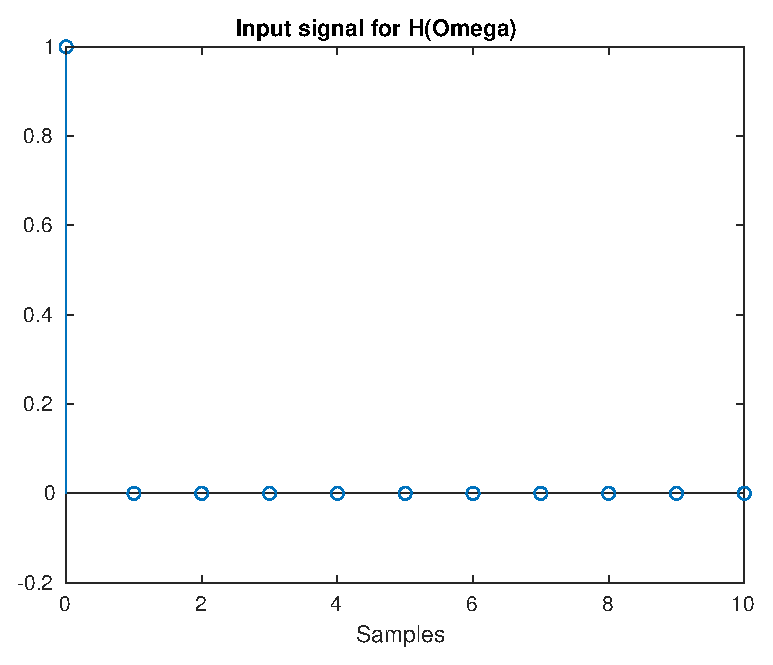
\includegraphics [width=4in]{hw5_11.eps}

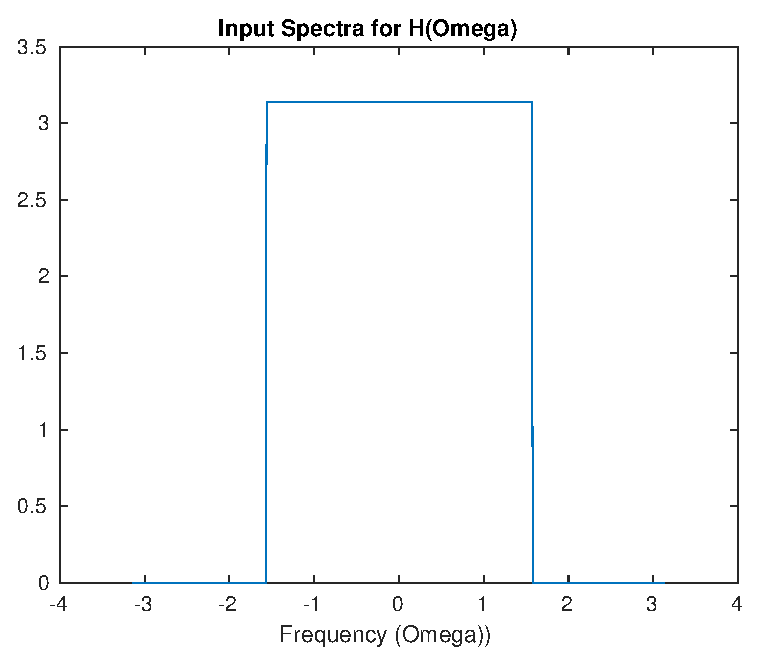
\includegraphics [width=4in]{hw5_12.eps}

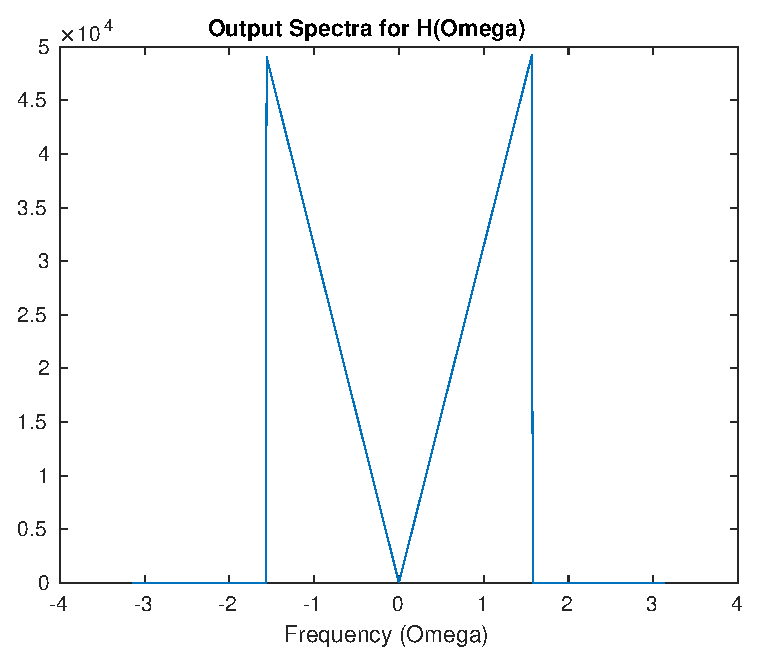
\includegraphics [width=4in]{hw5_13.eps}

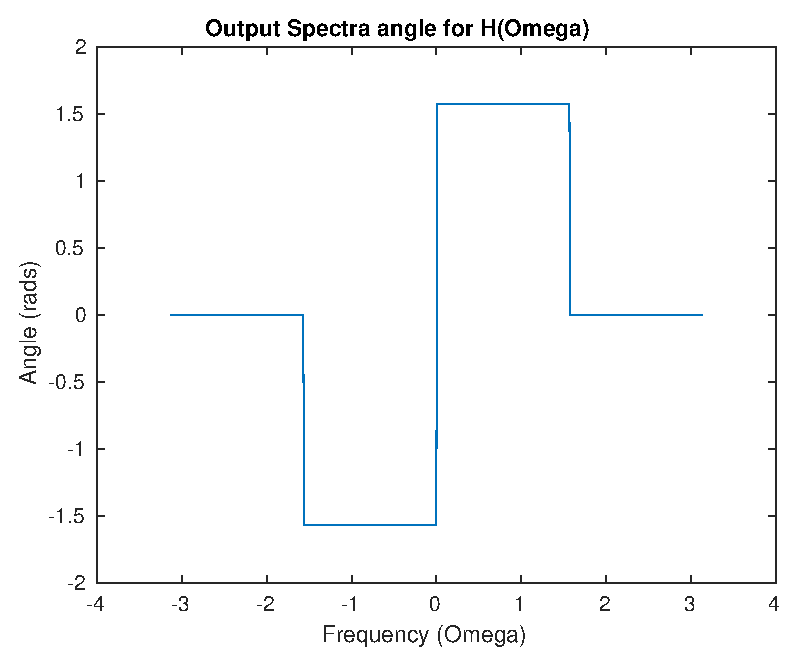
\includegraphics [width=4in]{hw5_14.eps}

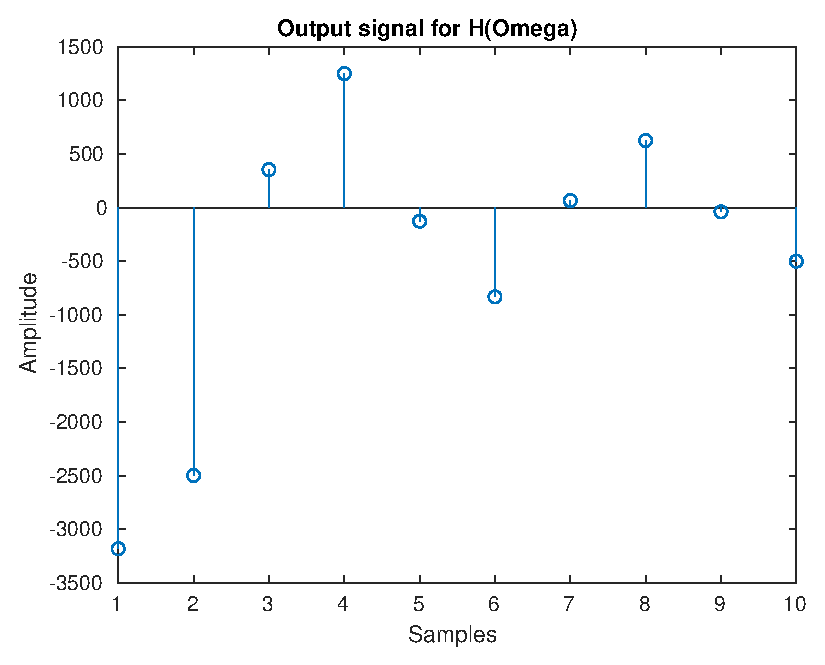
\includegraphics [width=4in]{hw5_15.eps}

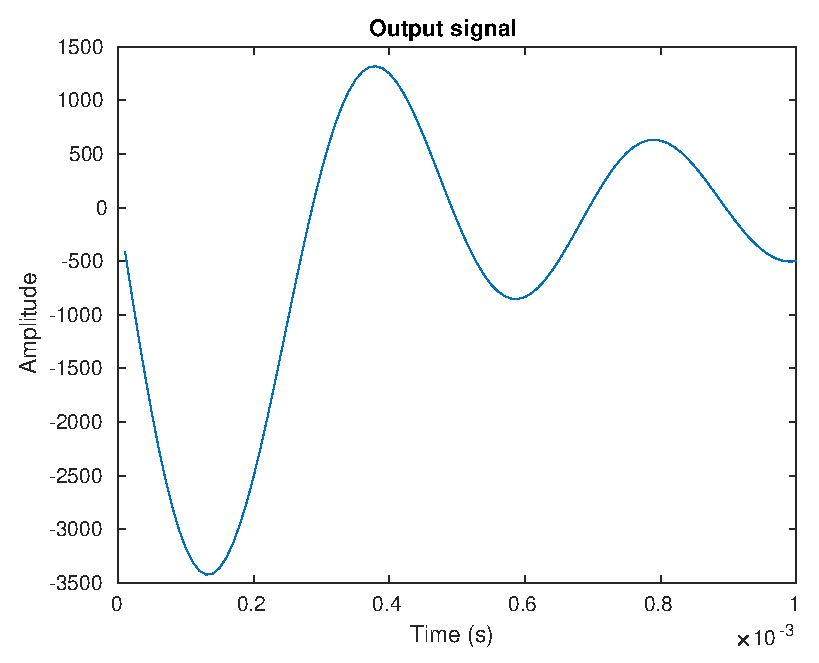
\includegraphics [width=4in]{hw5_16.eps}


\subsection*{DSP Homework 5 PRoblem 9 7.7-2}

\begin{verbatim}
Fs9 = 100/pi;
T9 = 1/Fs9;

% Part A
Omega9 = 0:.01:pi/2;

b1 = 0.03273793724;
b2 = 0.01799913516;
b3 = 0.00399530100;
a1a = -1.81915463768;
a1b = 0.95522952077;
a2a = -1.80572713311;
a2b = 0.88054034430;
a3a = -1.821397927591;
a3b = 0.83800435313;


b12 = conv([1 2 1],[1 2 1]);
ball = conv([b12],[1 2 1])
bi = b1*b2*b3;

a12 = conv([1 a1a a1b],[1 a2a a2b]);
aall = conv([a12],[1 a3a a3b]);

H9z = @(z) bi*(1 + ball(2)*z.^-1 + ball(3)*z.^-2 + ball(4)*z.^-3 + ...
    ball(5)*z.^-4 + ball(6)*z.^-5 + ball(7)*z.^-6)./(1 + aall(2)*z.^-1 ...
    + aall(3)*z.^-2 + aall(4)*z.^-3 + aall(5)*z.^-4 + aall(6)*z.^-5 + aall(7)*z.^-6);


H9ztf = tf(bi*ball,aall)

% Part B
figure;
plot(Omega9./T9, abs(H9z(exp(Omega9*j))));
title('Magnitude of H(z) Expanded');
xlabel('Frequency (Omega)');
ylabel('Amplitude');
% bode(H9ztf);

i = 1;
barray(4,1) = 0;
aarray(4,7) = 0;
bQF(4,1)    = 0;
aQF(4,1)    = 0;
bits(4,1)   = 0;


% Part C
for q = 12:-2:6
    for n = 1:32
        bSearch = round(bi*2^n);
        if abs(bSearch*20) > 2^(q - 2) && abs(bSearch*20) < 2^(q - 1)
            barray(i,1) = bSearch;
            bQF(i,1) = -n;
        end
        aSearch = round(aall(4)*2^n);
        if abs(aSearch) > 2^(q -2) && abs(aSearch) < 2^(q - 1)
            for k = 1:7
                aarray(i,k) = round(aall(k)*2^n);
            end
            aQF(i,1)    = -n;
        end
    end
    bits(i,1) = q;
    i = i + 1;
end

totalArray = cat(2, bits, barray, bQF, aarray, aQF)
coefTable = array2table(totalArray, 'VariableNames', {'Quant_bit','b0', 'b_2_Scale_Fac', ...
    'a0','a1','a2','a3','a4','a5','a6','a_2_Scale_Fac'})

for k = 1:4
    figure;
    b0Sauce = barray(k)*2^(bQF(k));
    aSauce = 2^(aQF(k));
    zplane([b0Sauce b0Sauce*ball(2) b0Sauce*ball(3) b0Sauce*ball(4) b0Sauce*ball(5) ...
        b0Sauce*ball(6) b0Sauce*ball(7)],[aSauce*aarray(k,1) aSauce*aarray(k,2) ...
        aSauce*aarray(k,3) aSauce*aarray(k,4) aSauce*aarray(k,5) aSauce*aarray(k,6) ...
        aSauce*aarray(k,7)]);
    title(['Pole-Zero plot for quantization ' num2str(bits(k)) ' bits']);

end

figure;
zplane([ball(1) ball(2) ball(3) ball(4) ball(5) ball(6) ball(7)], ...
    [aall(1) aall(2) aall(3) aall(4) aall(5) aall(6) aall(7)]);
title('Original Pole-Zero plot before quantization');

for k = 1:4
    H9zQuantized = @(z) barray(k)*2^(bQF(k)).*(1 + ball(2)*z.^-1 + ball(3)*z.^-2 + ball(4)*z.^-3 + ...
        ball(5)*z.^-4 + ball(6)*z.^-5 + ball(7)*z.^-6)./(2^(aQF(k))*(aarray(k,1) + aarray(k,2)*z.^-1 ...
        + aarray(k,3)*z.^-2 + aarray(k,4)*z.^-3 + aarray(k,5)*z.^-4 + aarray(k,6)*z.^-5 + aarray(k,7)*z.^-6));

    figure;
    plot(Omega9, abs(H9zQuantized(exp(j*Omega9))));
    title(['Magnitude plot for quantization ' num2str(bits(k)) ' bits']);
    xlabel('Frequency (Omega)');
end

i = 1;
barray2(10,1) = 0;
aarray2(10,7) = 0;
bQF2(10,1)    = 0;
aQF2(10,1)    = 0;
bits2(10,1)   = 0;

for q = 15:24
    for n = 1:256
        bSearch = round(bi*2^n);
        if abs(bSearch*20) > 2^(q - 2) && abs(bSearch*20) < 2^(q - 1)
            barray2(i,1) = bSearch;
            bQF2(i,1) = -n;
        end
        aSearch = round(aall(4)*2^n);
        if abs(aSearch) > 2^(q -2) && abs(aSearch) < 2^(q - 1)
            for k = 1:7
                aarray2(i,k) = round(aall(k)*2^n);
            end
            aQF2(i,1)    = -n;
        end
    end
    bits2(i,1) = q;
    i = i + 1;
end

for k = 1:10
    figure;
    b0Sauce2 = barray2(k)*2^(bQF2(k));
    aSauce2 = 2^(aQF2(k));
    zplane([b0Sauce2 b0Sauce2*ball(2) b0Sauce2*ball(3) b0Sauce2*ball(4) b0Sauce2*ball(5) ...
        b0Sauce2*ball(6) b0Sauce2*ball(7)],[aSauce2*aarray2(k,1) aSauce2*aarray2(k,2) ...
        aSauce2*aarray2(k,3) aSauce2*aarray2(k,4) aSauce2*aarray2(k,5) aSauce2*aarray2(k,6) ...
        aSauce2*aarray2(k,7)]);
    title(['Pole-Zero plot for quantization ' num2str(bits2(k)) ' bits']);

end
\end{verbatim}

        \color{lightgray} \begin{verbatim}
ball =

     1     6    15    20    15     6     1


H9ztf =
 
                                                                          
  2.354e-06 s^6 + 1.413e-05 s^5 + 3.531e-05 s^4 + 4.708e-05 s^3           
                                                                          
                                 + 3.531e-05 s^2 + 1.413e-05 s + 2.354e-06
                                                                          
  ------------------------------------------------------------------------
                                                                        
   s^6 - 5.446 s^5 + 12.56 s^4 - 15.69 s^3 + 11.19 s^2 - 4.32 s + 0.7049
                                                                        
 
Continuous-time transfer function.


totalArray =

  Columns 1 through 6

          12          79         -25         128        -697        1608
          10          20         -23          32        -174         402
           8           5         -21           8         -44         100
           6           1         -19           2         -11          25

  Columns 7 through 11

       -2008        1433        -553          90          -7
        -502         358        -138          23          -5
        -126          90         -35           6          -3
         -31          22          -9           1          -1


coefTable =

  4×11 table

    Quant_bit    b0    b_2_Scale_Fac    a0      a1      a2      a3       a4      a5     a6    a_2_Scale_Fac
    _________    __    _____________    ___    ____    ____    _____    ____    ____    __    _____________

       12        79         -25         128    -697    1608    -2008    1433    -553    90         -7      
       10        20         -23          32    -174     402     -502     358    -138    23         -5      
        8         5         -21           8     -44     100     -126      90     -35     6         -3      
        6         1         -19           2     -11      25      -31      22      -9     1         -1      

\end{verbatim} \color{black}
    
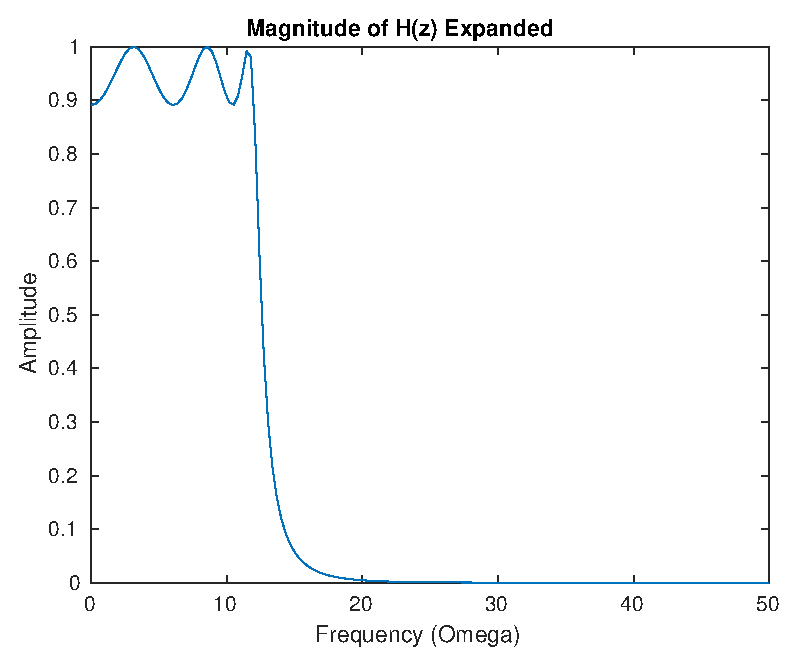
\includegraphics [width=4in]{hw5_17.eps}

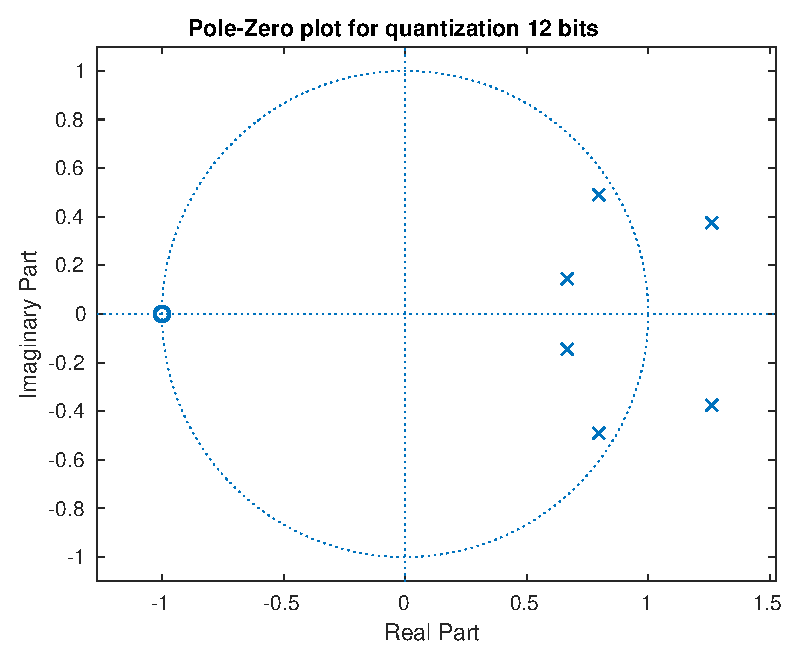
\includegraphics [width=4in]{hw5_18.eps}

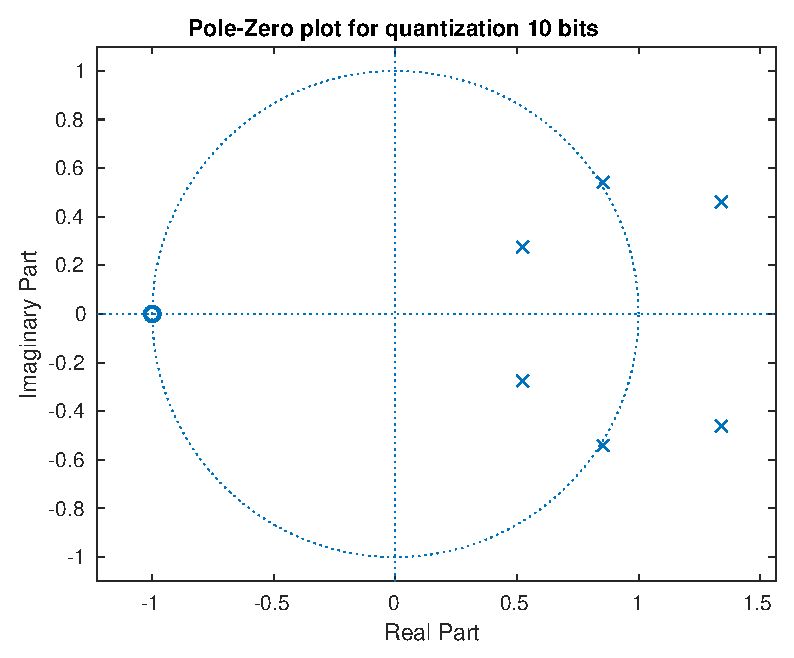
\includegraphics [width=4in]{hw5_19.eps}

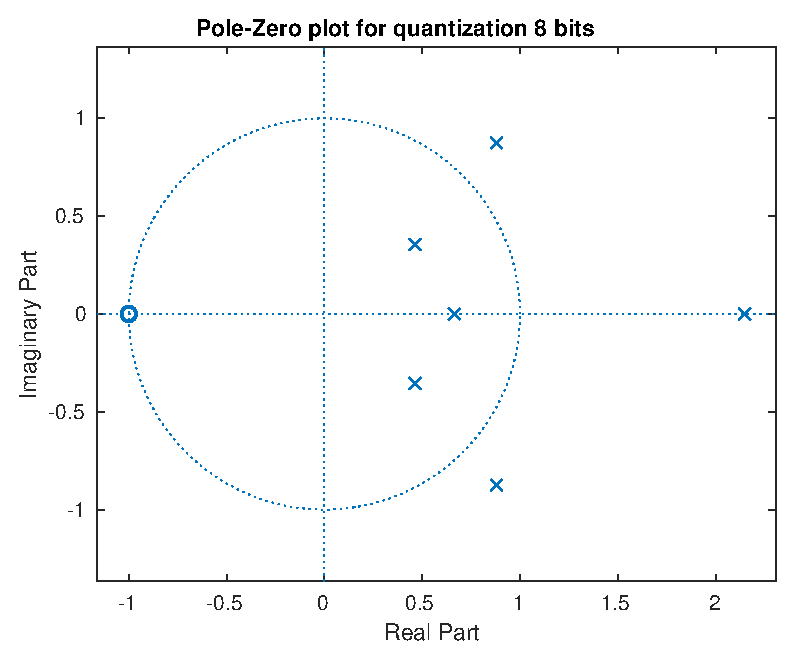
\includegraphics [width=4in]{hw5_20.eps}

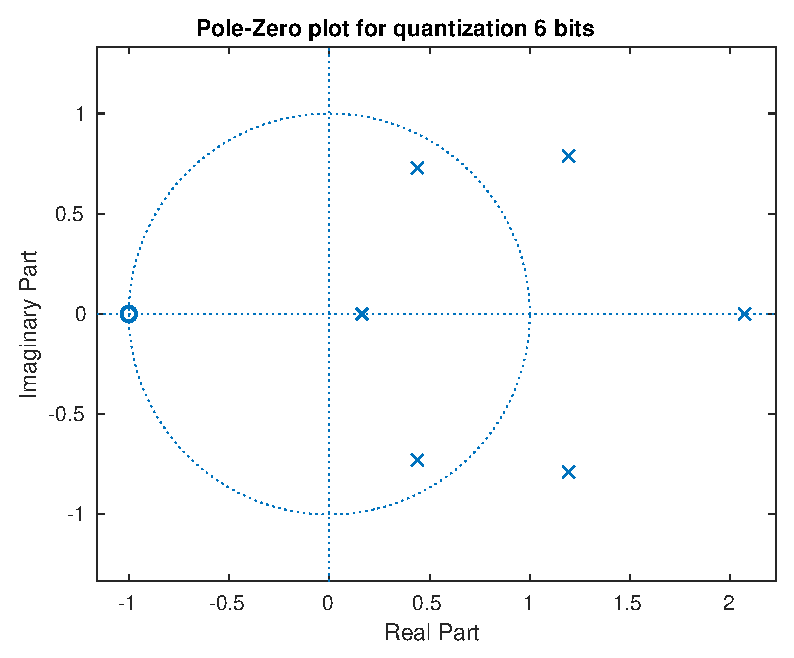
\includegraphics [width=4in]{hw5_21.eps}

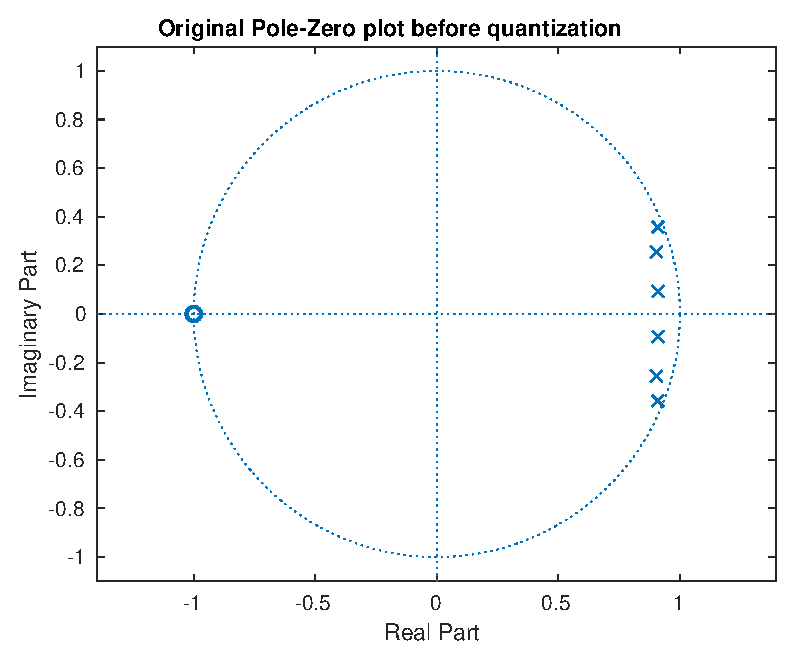
\includegraphics [width=4in]{hw5_22.eps}

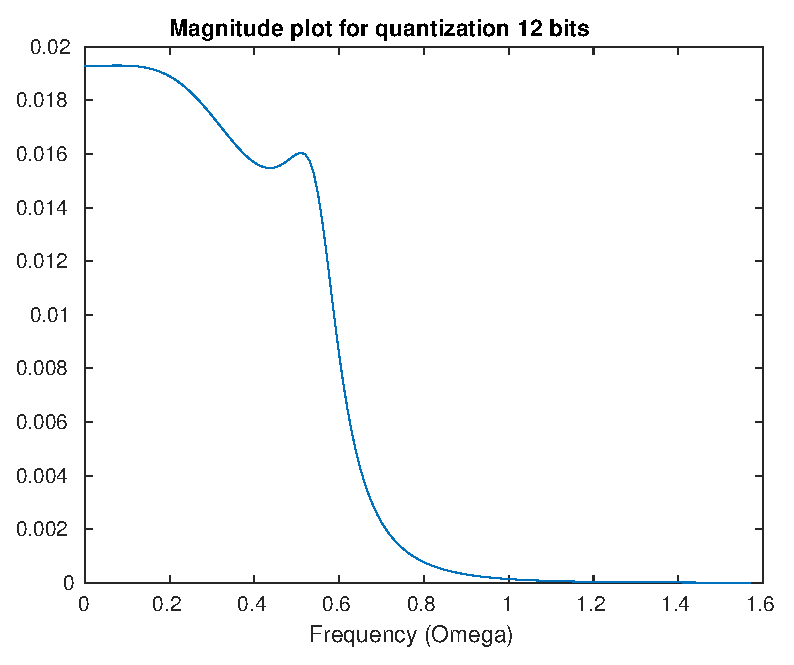
\includegraphics [width=4in]{hw5_23.eps}

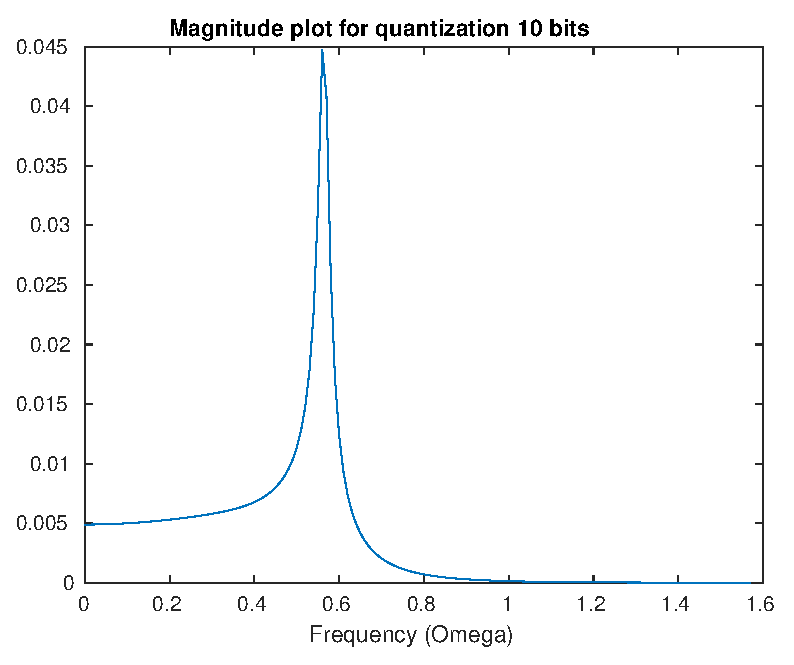
\includegraphics [width=4in]{hw5_24.eps}

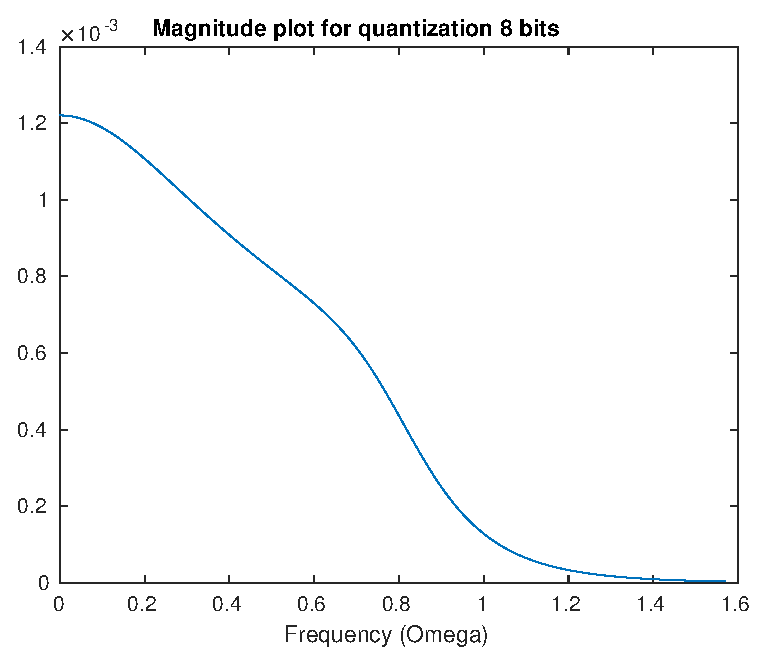
\includegraphics [width=4in]{hw5_25.eps}

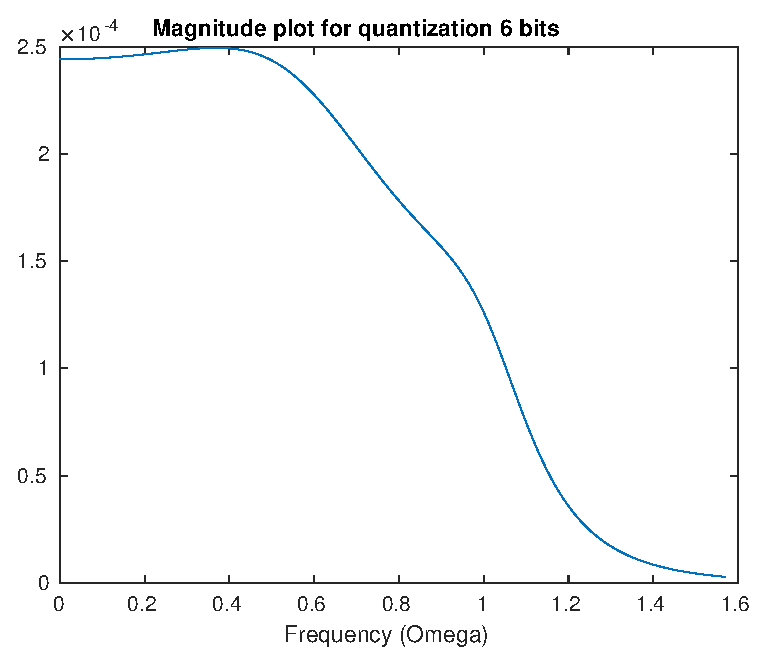
\includegraphics [width=4in]{hw5_26.eps}

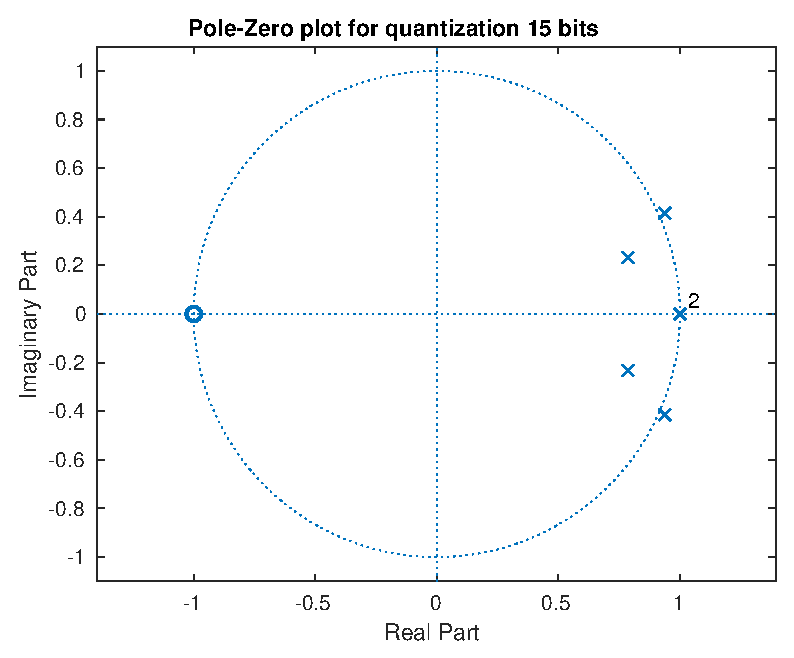
\includegraphics [width=4in]{hw5_27.eps}

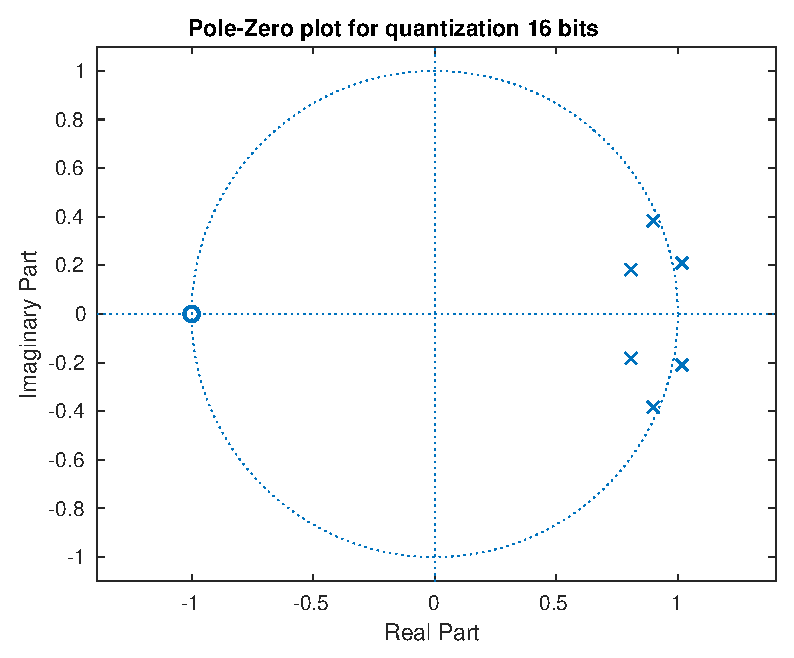
\includegraphics [width=4in]{hw5_28.eps}

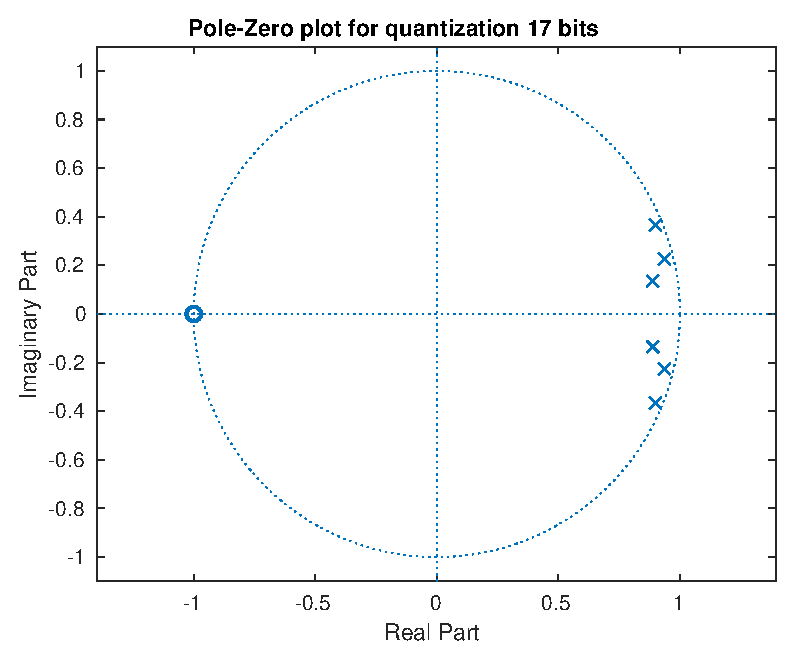
\includegraphics [width=4in]{hw5_29.eps}

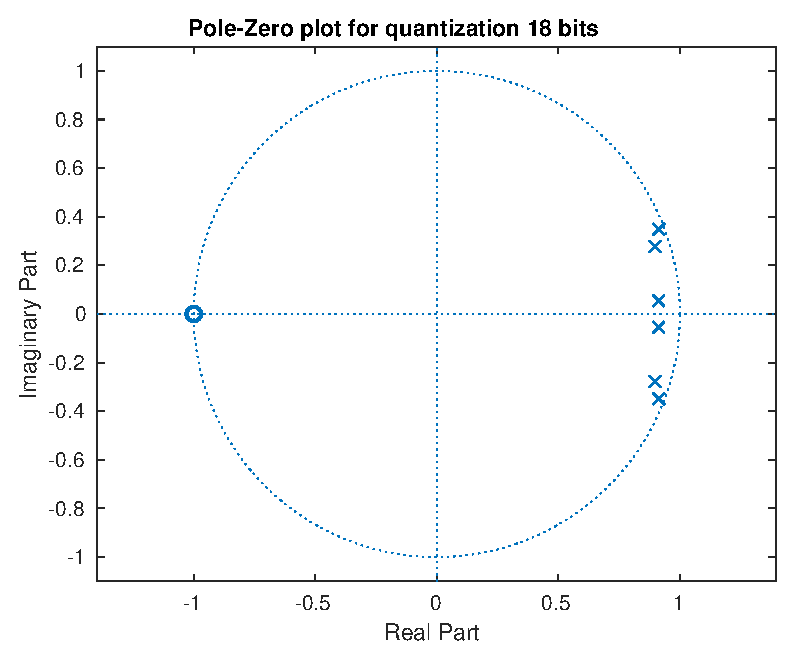
\includegraphics [width=4in]{hw5_30.eps}

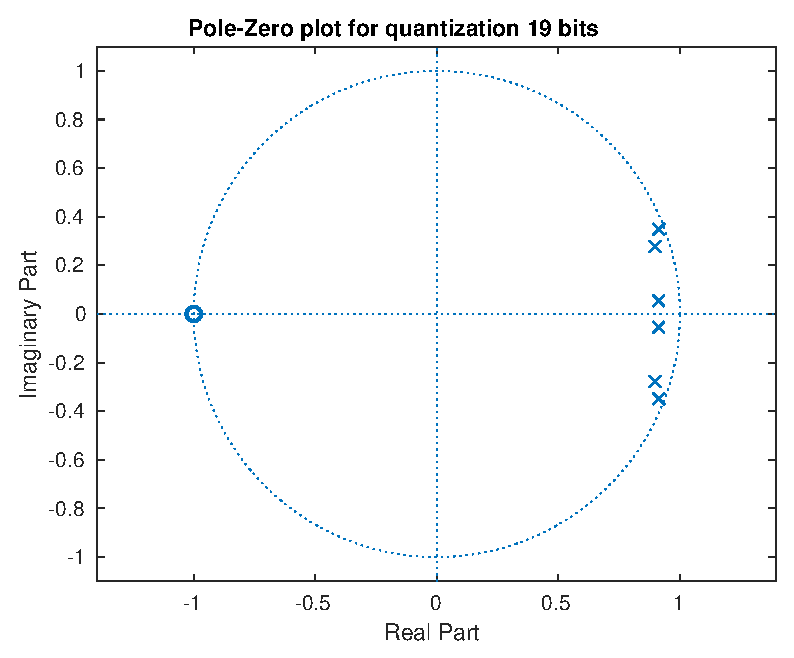
\includegraphics [width=4in]{hw5_31.eps}

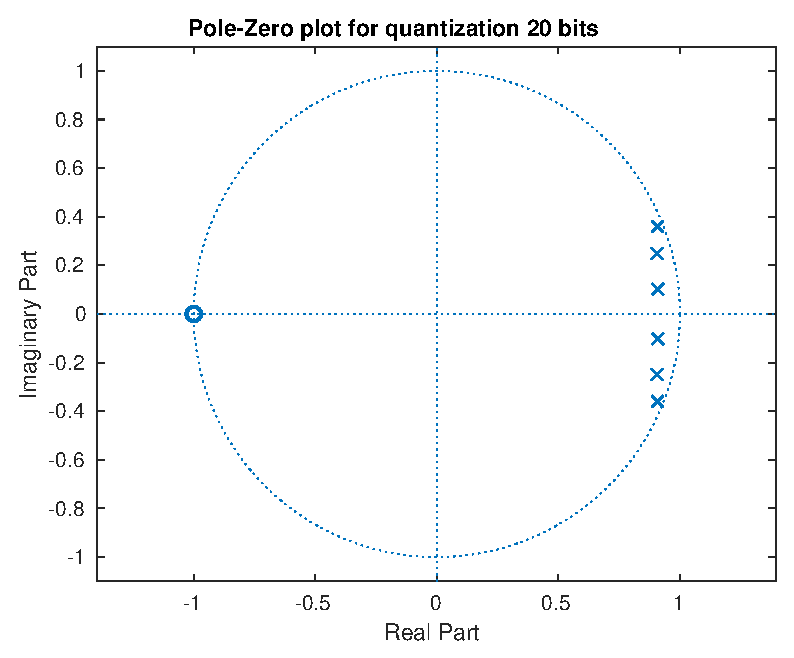
\includegraphics [width=4in]{hw5_32.eps}

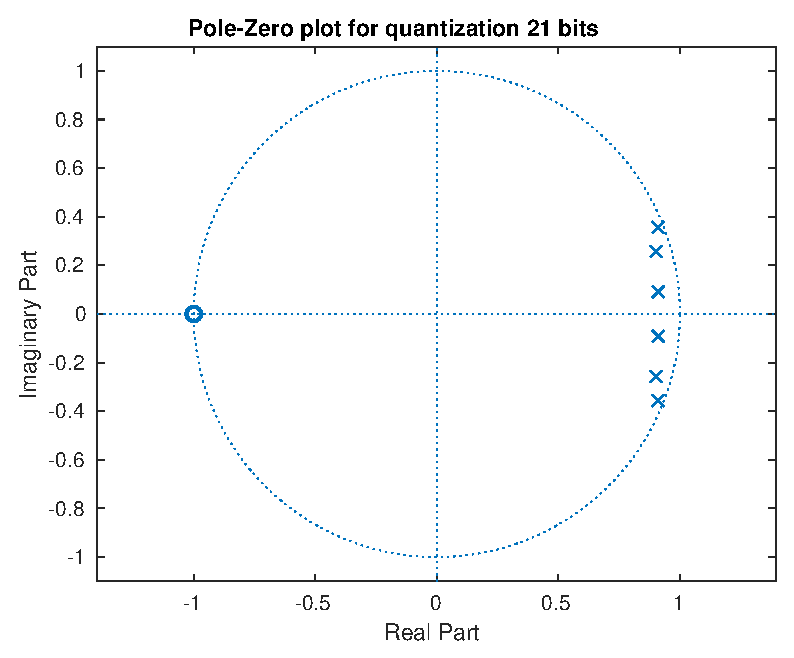
\includegraphics [width=4in]{hw5_33.eps}

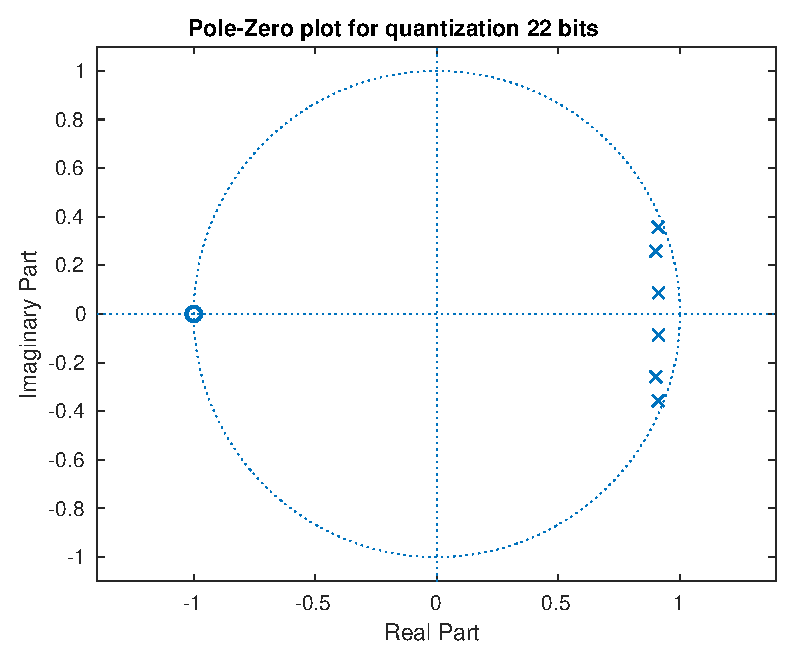
\includegraphics [width=4in]{hw5_34.eps}

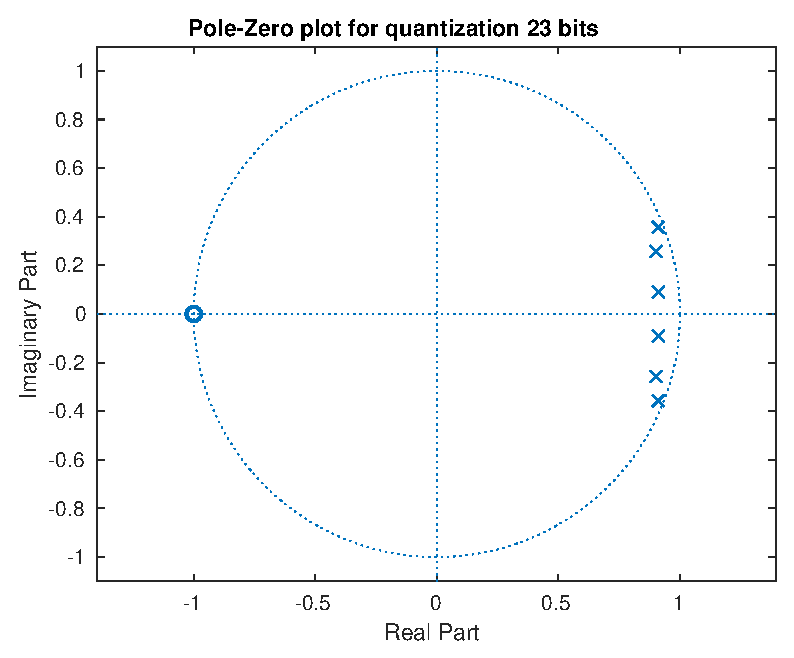
\includegraphics [width=4in]{hw5_35.eps}

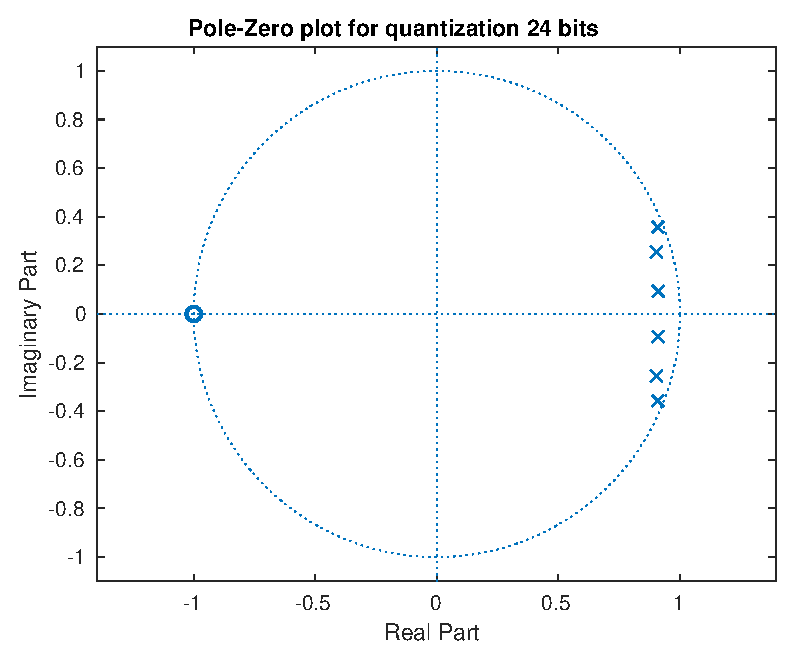
\includegraphics [width=4in]{hw5_36.eps}



\end{document}
    
